\documentclass{article}[18pt]
\usepackage[utf8]{inputenc}
\usepackage[margin=0.7in]{geometry}
\usepackage{parselines} 
\usepackage{amsmath}
\usepackage{titlesec}
\usepackage{pgfplots}
\usepackage{graphicx}
\usepackage[english]{babel}
\usepackage{fancyhdr}
\usetikzlibrary{decorations, decorations.text,positioning,quotes,arrows.meta,decorations.markings,3d,shapes}

\pgfplotsset{width=10cm,compat=1.9}

\titlespacing\section{0pt}{14pt plus 4pt minus 2pt}{0pt plus 2pt minus 2pt}
\newlength\tindent
\setlength{\tindent}{\parindent}
\setlength{\parindent}{0pt}
\renewcommand{\indent}{\hspace*{\tindent}}

\pagestyle{fancy}
\fancyhf{}
\rhead{Sam Robbins 13SE}
\lhead{A Level Physics - Fields}
\rfoot{Page \thepage}


\tikzstyle{arrow} = [thick,->,>=stealth]



\begin{document}
\begin{center}
\underline{\huge Electromagnetic Induction}
\end{center}
\section{Generating Electricity}
$ $\\
$ $\\

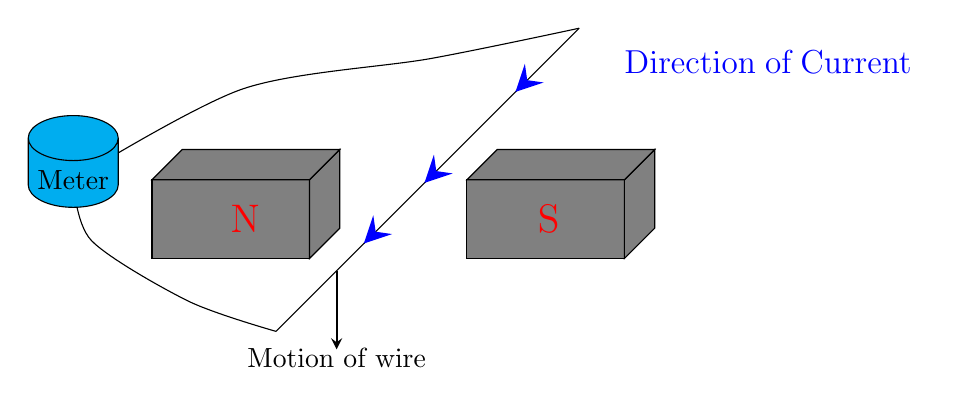
\begin{tikzpicture}
\tikzset{myptr/.style={decoration={markings,mark=at position 1 with %
    {\arrow[scale=3,>=stealth,blue]{>}}},postaction={decorate}}}
\pgfmathsetmacro{\cubex}{2}
\pgfmathsetmacro{\cubey}{1}
\pgfmathsetmacro{\cubez}{1}
\draw[black,fill=gray] (0,0,0) -- ++(-\cubex,0,0) -- ++(0,-\cubey,0) -- ++(\cubex,0,0) -- cycle;
\draw[black,fill=gray] (0,0,0) -- ++(0,0,-\cubez) -- ++(0,-\cubey,0) -- ++(0,0,\cubez) -- cycle;
\draw[black,fill=gray] (0,0,0) -- ++(-\cubex,0,0) -- ++(0,0,-\cubez) -- ++(\cubex,0,0) -- cycle;

\draw[black,fill=gray] (4,0,0) -- ++(-\cubex,0,0) -- ++(0,-\cubey,0) -- ++(\cubex,0,0) -- cycle;
\draw[black,fill=gray] (4,0,0) -- ++(0,0,-\cubez) -- ++(0,-\cubey,0) -- ++(0,0,\cubez) -- cycle;
\draw[black,fill=gray] (4,0,0) -- ++(-\cubex,0,0) -- ++(0,0,-\cubez) -- ++(\cubex,0,0) -- cycle;


\coordinate  (d5) at (1.5,0,5){};
\coordinate  (d6) at (1.5,0,-5){};

\draw []       (d5)--(d6);
\node[text width=4cm,red] at (1,-0.5) {\Large{N}};
\node[text width=4cm,red] at (4.9,-0.5) {\Large{S}};
\draw [arrow] (1.5,0,3) -- node[anchor=west,below,yshift=-10] {Motion of wire} (1.5,-1,3);
\draw [myptr] (1.5,0,-3) -- (1.5,0,-2.9);
\draw [myptr] (1.5,0,0) -- (1.5,0,0.1);
\draw [myptr] (1.5,0,2) -- (1.5,0,2.1);
\node[text width=4cm,blue] at (6,1.5) {\large{Direction of Current}};
\draw [black] plot [smooth] coordinates { (1.5,0,5) (0,0,4) (-2,0,2) (-3,0,0)};
\draw [black] plot [smooth] coordinates { (1.5,0,-5) (0,0,-4) (-2,0,-3) (-3,0,0)};
\node[cylinder, draw, shape aspect=.5,shape border rotate=90,fill=cyan] at (-3,0) {Meter};
\end{tikzpicture}
\end{document}